% Presentacion oral (10 minutos de exposicion). Compilar desde esta carpeta: pdflatex presentacion.tex
% Formato 16:9, una diapositiva por pagina. Las cifras salen de los mismos archivos que el informe.
% Tiempo sugerido: portada 0:15 | 2-7 punto 1, unos 4:30 | 8-12 punto 2, unos 4:30 | 13 cierre 0:45
\documentclass[12pt]{article}
\usepackage[utf8]{inputenc}
\usepackage[T1]{fontenc}
\usepackage[spanish,es-nodecimaldot,es-noshorthands]{babel}
\usepackage{newtxtext,newtxmath}
\usepackage{graphicx}
\usepackage{xcolor}
\usepackage{amsmath}
\usepackage{tikz}
\usepackage{fancyhdr}
\usepackage{enumitem}
\usepackage[paperwidth=25.4cm,paperheight=14.29cm,left=1.1cm,right=1.1cm,top=0.6cm,bottom=1.1cm,footskip=0.55cm]{geometry}
% Generado por codigo/punto1/cifras_punto1.py. No editar a mano.
\newcommand{\EToAnual}{1179}
\newcommand{\EToMesMin}{86}
\newcommand{\EToMesMax}{110}
\newcommand{\DifPromMax}{0{,}30}
\newcommand{\DifPuntoMax}{1{,}58}
\newcommand{\DzMin}{$-$806}
\newcommand{\DzMax}{394}
\newcommand{\DzPond}{18}
\newcommand{\CobEra}{90{,}1}
\newcommand{\PmQfis}{605}
\newcommand{\EToFis}{1182}
\newcommand{\TCr}{0{,}90}
\newcommand{\TCsesgo}{1{,}4}
\newcommand{\TCmae}{4{,}0}
\newcommand{\PIr}{0{,}70}
\newcommand{\PIsesgo}{$-$1{,}0}
\newcommand{\PImae}{8{,}0}
\newcommand{\NOr}{0{,}81}
\newcommand{\NOsesgo}{4{,}7}
\newcommand{\NOmae}{11{,}1}
\newcommand{\MAEThorn}{38{,}7}
\newcommand{\SesgoThorn}{$-$39}
\newcommand{\RThorn}{0{,}57}
\newcommand{\MAEHarg}{6{,}1}
\newcommand{\SesgoHarg}{$-$6}
\newcommand{\RHarg}{0{,}92}
\newcommand{\MAEPT}{20{,}2}
\newcommand{\SesgoPT}{21}
\newcommand{\RPT}{0{,}96}
\newcommand{\MAEMeyer}{58{,}6}
\newcommand{\SesgoMeyer}{$-$60}
\newcommand{\RMeyer}{0{,}56}
\newcommand{\MAEMakk}{5{,}0}
\newcommand{\SesgoMakk}{5}
\newcommand{\RMakk}{0{,}98}
\newcommand{\MAERohw}{53{,}9}
\newcommand{\SesgoRohw}{$-$55}
\newcommand{\RRohw}{0{,}54}
\newcommand{\FracRadMin}{83}
\newcommand{\FracRadMax}{92}
\newcommand{\AlfaMin}{1{,}00}
\newcommand{\AlfaMax}{1{,}09}
\newcommand{\VPDMin}{0{,}36}
\newcommand{\VPDMax}{0{,}68}
\newcommand{\SensRs}{$-$85}
\newcommand{\SensPctRs}{$-$7{,}2}
\newcommand{\SensTunoEa}{42}
\newcommand{\SensPctTunoEa}{3{,}6}
\newcommand{\SensTunoHR}{30}
\newcommand{\SensPctTunoHR}{2{,}5}
\newcommand{\SensTdosEa}{83}
\newcommand{\SensPctTdosEa}{7{,}0}
\newcommand{\SensTdosHR}{60}
\newcommand{\SensPctTdosHR}{5{,}1}
\newcommand{\SensEa}{$-$20}
\newcommand{\SensPctEa}{$-$1{,}7}
\newcommand{\SensUdos}{4}
\newcommand{\SensPctUdos}{0{,}3}
\newcommand{\SensThornTuno}{4{,}5}
\newcommand{\ETgleam}{740}
\newcommand{\ETmod}{796}
\newcommand{\ETbalL}{603}
\newcommand{\ETbalI}{73}
\newcommand{\SobreGleam}{23}
\newcommand{\SobreMod}{32}
\newcommand{\PL}{1104}
\newcommand{\Qmed}{501}
\newcommand{\DifPLPI}{530}
\newcommand{\SigmaP}{175}
\newcommand{\SigmaQ}{38}
\newcommand{\SigmaET}{180}
\newcommand{\SigmaETpct}{30}
\newcommand{\RnLambda}{1743}
\newcommand{\FEbal}{0{,}35}
\newcommand{\EToHumMin}{0{,}72}
\newcommand{\EToHumMax}{0{,}89}
\newcommand{\EToSecMin}{0{,}43}
\newcommand{\EToSecMax}{0{,}62}
\newcommand{\CorrFEg}{0{,}92}
\newcommand{\CorrFEm}{0{,}91}
\newcommand{\KnotG}{0{,}31}
\newcommand{\KnotM}{0{,}36}
\newcommand{\PhiAr}{1{,}08}
\newcommand{\EIg}{0{,}67}
\newcommand{\EIm}{0{,}72}
\newcommand{\OmG}{2{,}28}
\newcommand{\OmM}{2{,}59}
\newcommand{\BudyEI}{0{,}64}
\newcommand{\DistG}{0{,}03}
\newcommand{\DistM}{0{,}08}
\newcommand{\ElasG}{1{,}95}
\newcommand{\ElasM}{2{,}19}
\newcommand{\PhiI}{2{,}08}
\newcommand{\EToSeco}{1211}
\newcommand{\EToHumedo}{1173}
\newcommand{\ETSecoG}{707}
\newcommand{\ETHumG}{776}
\newcommand{\CorrPETo}{$-$0{,}75}
\newcommand{\TendETo}{1{,}14}
\newcommand{\pETo}{0{,}0026}
\newcommand{\TendTh}{0{,}57}
\newcommand{\pTh}{0{,}0005}
\newcommand{\TendT}{0{,}18}
\newcommand{\AtrT}{0{,}76}
\newcommand{\AtrEa}{$-$0{,}13}
\newcommand{\AtrUdos}{0{,}01}
\newcommand{\AtrRs}{0{,}57}
\newcommand{\AtrSuma}{1{,}21}
\newcommand{\AtrRes}{$-$0{,}05}
\newcommand{\EToBajo}{1307}
\newcommand{\EToAlto}{1083}
\newcommand{\GlBajo}{801}
\newcommand{\GlAlto}{604}
\newcommand{\ModBajo}{575}
\newcommand{\ModAlto}{813}
\newcommand{\ModMax}{889}
\newcommand{\ModMaxBanda}{2750-3250 m}

% Generado por codigo/punto2/analisis_final_punto2.py. No editar a mano.
\newcommand{\NAnios}{20}
\newcommand{\AreaMicro}{0{,}123}
\newcommand{\LongCauce}{382{,}7}
\newcommand{\PendCauce}{0{,}125}
\newcommand{\Cpre}{0{,}332}
\newcommand{\Cpremenos}{0{,}266}
\newcommand{\Cpremas}{0{,}399}
\newcommand{\Curb}{0{,}60}
\newcommand{\tcKirpich}{4{,}2}
\newcommand{\tcKerby}{21{,}5}
\newcommand{\tcSCS}{12{,}5}
\newcommand{\tcUrb}{7{,}6}
\newcommand{\Tdis}{25}
\newcommand{\Vida}{30}
\newcommand{\RiesgoNom}{70{,}6}
\newcommand{\RiesgoAcept}{75}
\newcommand{\Treq}{22{,}1}
\newcommand{\Idis}{129{,}8}
\newcommand{\Qp}{1{,}476}
\newcommand{\Dcalc}{0{,}83}
\newcommand{\Dcom}{0{,}90}
\newcommand{\Qcap}{1{,}81}
\newcommand{\FS}{1{,}23}
\newcommand{\Drec}{1{,}05}
\newcommand{\QcapRec}{2{,}73}
\newcommand{\FSrec}{1{,}85}
\newcommand{\PeffRec}{1{,}05}
\newcommand{\TeffRec}{95}
\newcommand{\RiesgoEffRec}{27{,}2}
\newcommand{\Peff}{4{,}97}
\newcommand{\Teff}{20}
\newcommand{\RiesgoEff}{78{,}3}
\newcommand{\ProbQLQc}{30{,}8}
\newcommand{\QLlo}{0{,}92}
\newcommand{\QLhi}{2{,}69}
\newcommand{\Dlo}{0{,}70}
\newcommand{\Dhi}{1{,}04}
\newcommand{\NMC}{5000}
\newcommand{\NBoot}{500}
\newcommand{\WeissDiez}{1{,}143}
\newcommand{\WeissHora}{1{,}021}
\newcommand{\QdiezTcien}{32{,}7}
\newcommand{\QhoraTcien}{69{,}7}
\newcommand{\KosHoraTcien}{45{,}9}
\newcommand{\RazonHoraTcien}{1{,}52}
\newcommand{\KosUCHoraTcien}{26}
\newcommand{\SinHoraTcien}{55{,}5}
\newcommand{\RazonDiezTveinte}{1{,}12}
\newcommand{\IDFtheta}{0{,}120}
\newcommand{\IDFeta}{0{,}828}
\newcommand{\IDFrmse}{1{,}8}
\newcommand{\IDFerr}{11{,}1}
\newcommand{\IDFrdos}{0{,}999}
\newcommand{\Qpre}{1{,}476}
\newcommand{\DOrif}{0{,}701}
\newcommand{\Cd}{0{,}61}
\newcommand{\Hutil}{2{,}0}
\newcommand{\VolCrit}{1350}
\newcommand{\EscCrit}{bloques alternos + tiempo-area, pico al centro}
\newcommand{\LadoTanque}{26{,}0}
\newcommand{\VolUtil}{1352}
\newcommand{\VolTrap}{993}
\newcommand{\TrapCrit}{d=15 min}
\newcommand{\VolInicio}{979}
\newcommand{\VolCentro}{1350}
\newcommand{\VolFinal}{1288}
\newcommand{\QsalMax}{1{,}475}
\newcommand{\TeventoTrece}{196}
\newcommand{\TeventoVeintiuno}{28{,}1}
\newcommand{\TeventoVeintiunoLo}{8{,}4}
\newcommand{\TeventoVeintiunoHi}{3265}
\newcommand{\AnchoTcien}{57}
\newcommand{\CompletMin}{98{,}54}

% Generado por codigo/punto2/contraste_evento_2013.py
\newcommand{\EvRadarEst}{33{,}8}
\newcommand{\EvRadarTresEst}{45{,}8}
\newcommand{\EvRadarMaxVent}{67{,}8}
\newcommand{\EvAreaCuarenta}{168}
\newcommand{\EvBuhler}{59{,}5}
\newcommand{\EvNeubronn}{34{,}6}
\newcommand{\EvGoggingen}{27{,}7}
\newcommand{\EvAalen}{12{,}9}
\newcommand{\EvHeubach}{11{,}5}
\newcommand{\EvGmundHora}{17{,}1}
\newcommand{\EvEllwHora}{7{,}6}
\newcommand{\EvGmundDia}{22{,}2}
\newcommand{\EvGmundKm}{17}
\newcommand{\EvEllwKm}{18}
\newcommand{\EvBuhlerKm}{9}
\newcommand{\EvRadarBuhler}{33{,}2}
\newcommand{\VecGmundAnios}{23}
\newcommand{\VecEllwAnios}{23}
\newcommand{\VecGmundComp}{98{,}9}
\newcommand{\VecEllwComp}{99{,}5}
\newcommand{\VecGmundQcien}{59{,}7}
\newcommand{\VecEllwQcien}{59{,}3}
\newcommand{\VecPropQcien}{69{,}8}
\newcommand{\VecRhoGmund}{0{,}30}
\newcommand{\VecRhoEllw}{0{,}21}

\graphicspath{{../../productos/punto1/}{../../productos/punto2/final/figuras/}{../../datos/punto2/Abtsgmuend_Untergroeningen/control_2_1/}}

\definecolor{acento}{RGB}{0,84,147}
\definecolor{tenue}{RGB}{110,110,110}
\definecolor{dato}{RGB}{190,60,20}
\setlength{\parindent}{0pt}
\setlist{nosep,leftmargin=1.2em,itemsep=7pt}
\pagestyle{fancy}
\fancyhf{}
\renewcommand{\headrulewidth}{0pt}
\fancyfoot[L]{\footnotesize\color{tenue}Tarea 2 · Hidrología 202602 · Grupo \textcolor{red}{GXX}}
\fancyfoot[R]{\footnotesize\color{tenue}\thepage}

% \slide{Etiqueta del apartado}{Mensaje principal de la diapositiva}
\newcommand{\slide}[2]{\newpage
  {\footnotesize\color{tenue}\MakeUppercase{#1}}\par\vspace{2pt}
  {\color{acento}\LARGE\bfseries #2}\par\vspace{4pt}
  {\color{acento}\rule{\linewidth}{0.8pt}}\par\vspace{0.35cm}}
\newcommand{\cifra}[2]{{\color{dato}\Huge\bfseries #1}\\[-2pt]{\small\color{tenue}#2}}
\renewcommand{\Large}{\fontsize{19}{24}\selectfont}
\renewcommand{\large}{\fontsize{16}{20}\selectfont}

\begin{document}
\thispagestyle{empty}
\vspace*{1.8cm}
{\color{acento}\fontsize{32}{38}\selectfont\bfseries Evapotranspiración\\[4pt] y diseño hidrológico}\par
\vspace{0.4cm}
{\color{acento}\rule{0.5\linewidth}{1.2pt}}\par\vspace{0.5cm}
{\Large Tarea 2 · Hidrología · Semestre 202602}\par\vspace{0.9cm}
{\large Andrés Francisco Idrobo Hidrobo\quad·\quad Enmaly Aleli Manturano Grajeda\quad·\quad Jeyson Cristian Javier Irpanoca}\par\vspace{0.25cm}
{\large\color{tenue} Grupo \textcolor{red}{GXX} · Profesor Carlos David Hoyos · Universidad Nacional de Colombia, Sede Medellín}

% ---------------------------------------------------------------- 2
\slide{Contexto}{Dos sitios, dos preguntas}
\begin{minipage}[t]{0.47\linewidth}
{\color{acento}\Large\bfseries Punto 1 · Racarumi, Perú}\\[6pt]
\Large ¿Cuánta agua devuelve la cuenca a la atmósfera, qué la limita y qué ha cambiado?\\[12pt]
\large 2363 km$^2$ · 264--4084 m\\
Lluvia \PL\ mm/año · caudal \Qmed\ mm/año\\
Temporada húmeda enero--abril
\end{minipage}\hfill
{\color{acento}\vrule width 0.8pt}\hfill
\begin{minipage}[t]{0.47\linewidth}
{\color{acento}\Large\bfseries Punto 2 · Abtsgmünd, Alemania}\\[6pt]
\Large ¿Qué lluvia debe soportar una alcantarilla y con qué riesgo real?\\[12pt]
\large DWD 00020 · lluvia cada 10 minutos\\
\NAnios\ años hidrológicos válidos (2006--2025)\\
Microcuenca de \AreaMicro\ km$^2$ a 414 m de la estación
\end{minipage}

% ---------------------------------------------------------------- 3
\slide{Punto 1 · Demanda atmosférica}{La demanda la controla la radiación, no la temperatura}
\begin{minipage}[c]{0.58\linewidth}
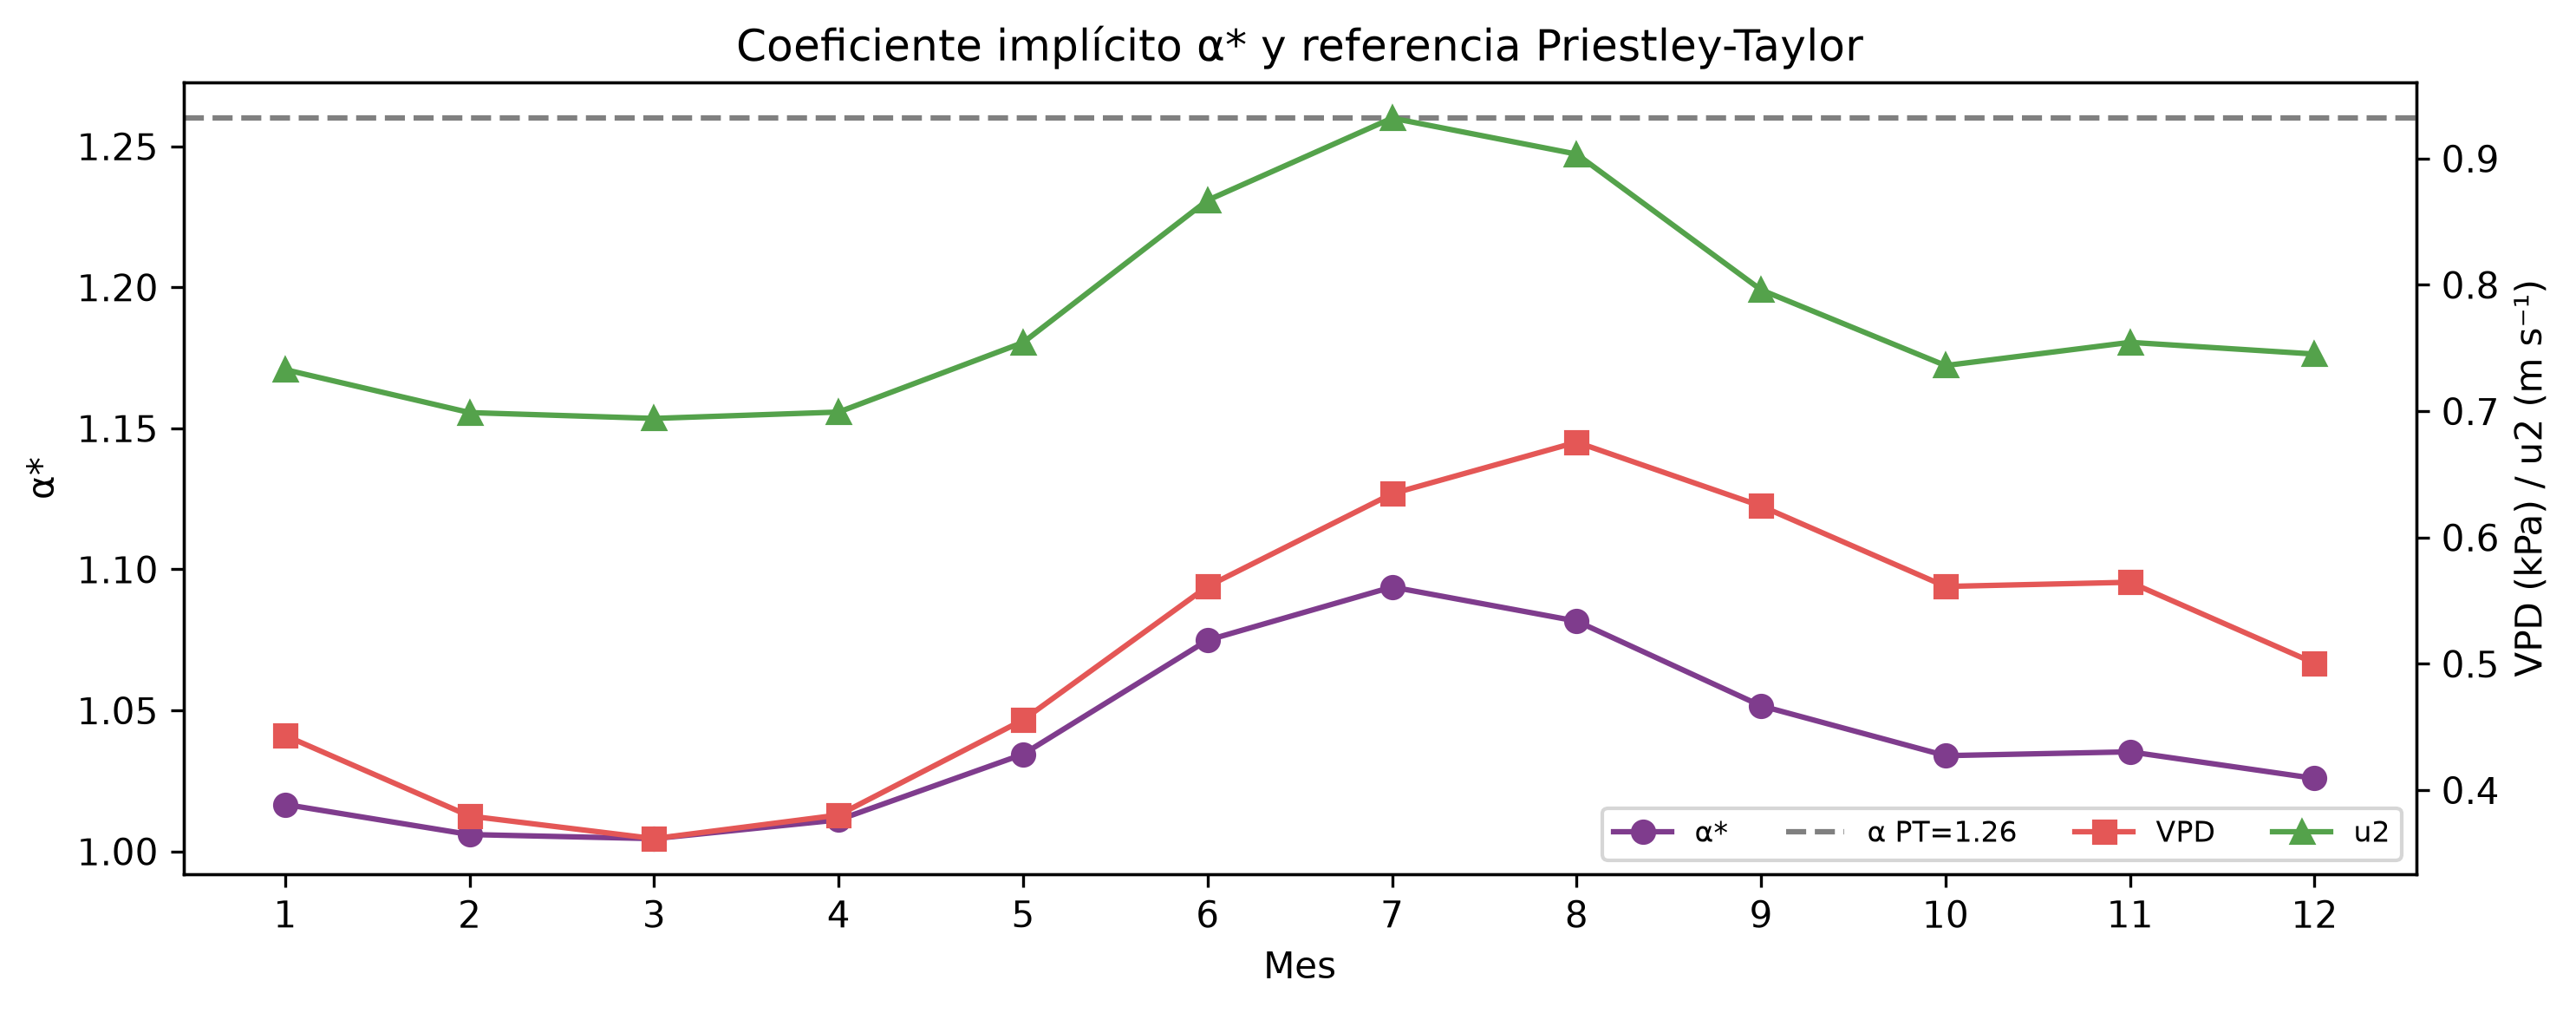
\includegraphics[width=\linewidth,height=0.72\textheight,keepaspectratio]{1_1_demanda_atmosferica/figuras/1_1d_alpha_star_vpd_viento.png}
\end{minipage}\hfill
\begin{minipage}[c]{0.38\linewidth}
\cifra{\EToAnual\ mm/año}{ETo FAO-56 (ERA5-Land, 90 \% de la cuenca)}\\[10pt]
\large
\begin{itemize}
\item Término radiativo: \FracRadMin--\FracRadMax\,\% de la ETo
\item $R_s-10$\,\%: \SensRs\ mm/año\\ $u_2+10$\,\%: +\SensUdos\ mm/año
\item $\alpha^*$ = \AlfaMin--\AlfaMax: poca advección
\end{itemize}
\end{minipage}

% ---------------------------------------------------------------- 4
\slide{Punto 1 · Métodos simples}{Los métodos radiativos siguen a FAO-56; Thornthwaite no}
\begin{minipage}[c]{0.55\linewidth}
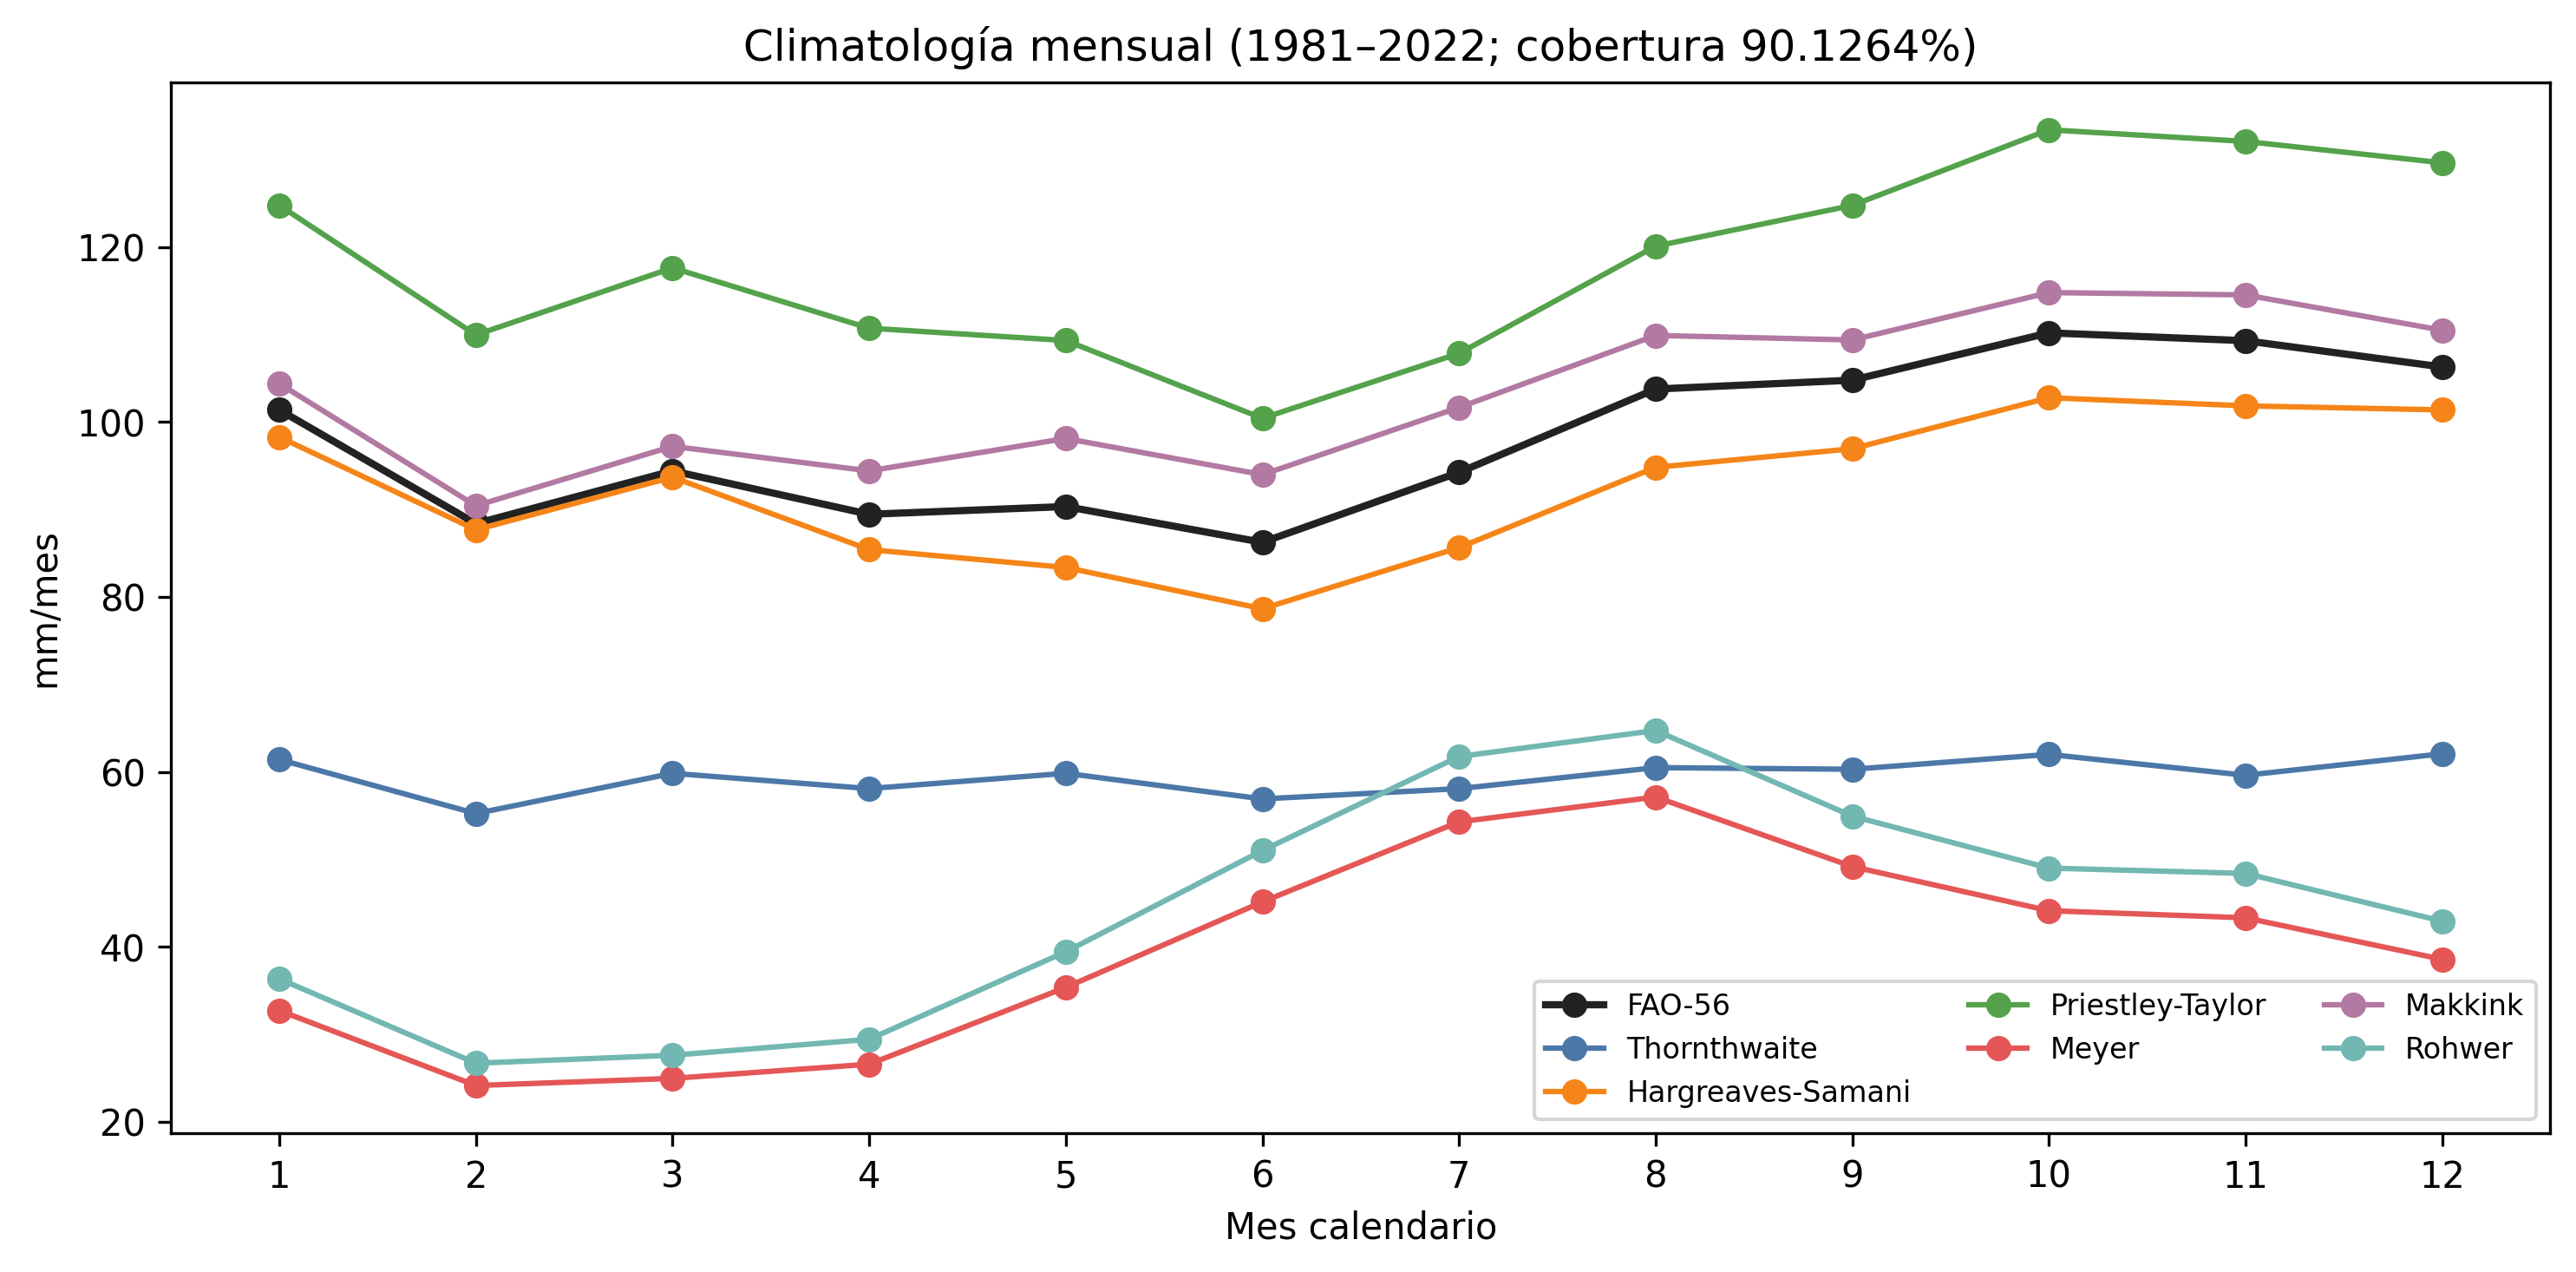
\includegraphics[width=\linewidth,height=0.72\textheight,keepaspectratio]{1_1_demanda_atmosferica/figuras/1_1c_climatologia_mensual.png}
\end{minipage}\hfill
\begin{minipage}[c]{0.41\linewidth}
\large
\begin{itemize}
\item Makkink: MAE \MAEMakk\ mm/mes, $r$ = \RMakk
\item Hargreaves calibrado (árbol de decisión, paso 4): MAE \MAEHarg\ $\to$ \HSmaeValCal\ mm/mes en validación
\item Thornthwaite: sesgo de \SesgoThorn\,\%; la temperatura tropical casi no cambia en el año
\item Ante +1 °C Thornthwaite sube \SensThornTuno\,\%, casi el doble que FAO-56
\end{itemize}
\end{minipage}

% ---------------------------------------------------------------- 5
\slide{Punto 1 · Evapotranspiración real}{La cuenca devuelve algo más de la mitad de su lluvia}
\begin{minipage}[c]{0.4\linewidth}
\cifra{\ETbalL\ $\pm$ \SigmaET\ mm/año}{Balance $P-Q$ con PISCOp (\SigmaETpct\,\% de incertidumbre)}\\[12pt]
\large
\begin{itemize}
\item La lluvia aporta \SigmaP\ de los \SigmaET\ mm de error
\item IMERG da \DifPLPI\ mm/año menos: inservible aquí
\item GLEAM \ETgleam\ y MOD16 \ETmod: +\SobreGleam\ a +\SobreMod\,\%
\item Hipótesis: lluvia subestimada en las cumbres y trasvases Chotano--Conchano
\end{itemize}
\end{minipage}\hfill
\begin{minipage}[c]{0.56\linewidth}
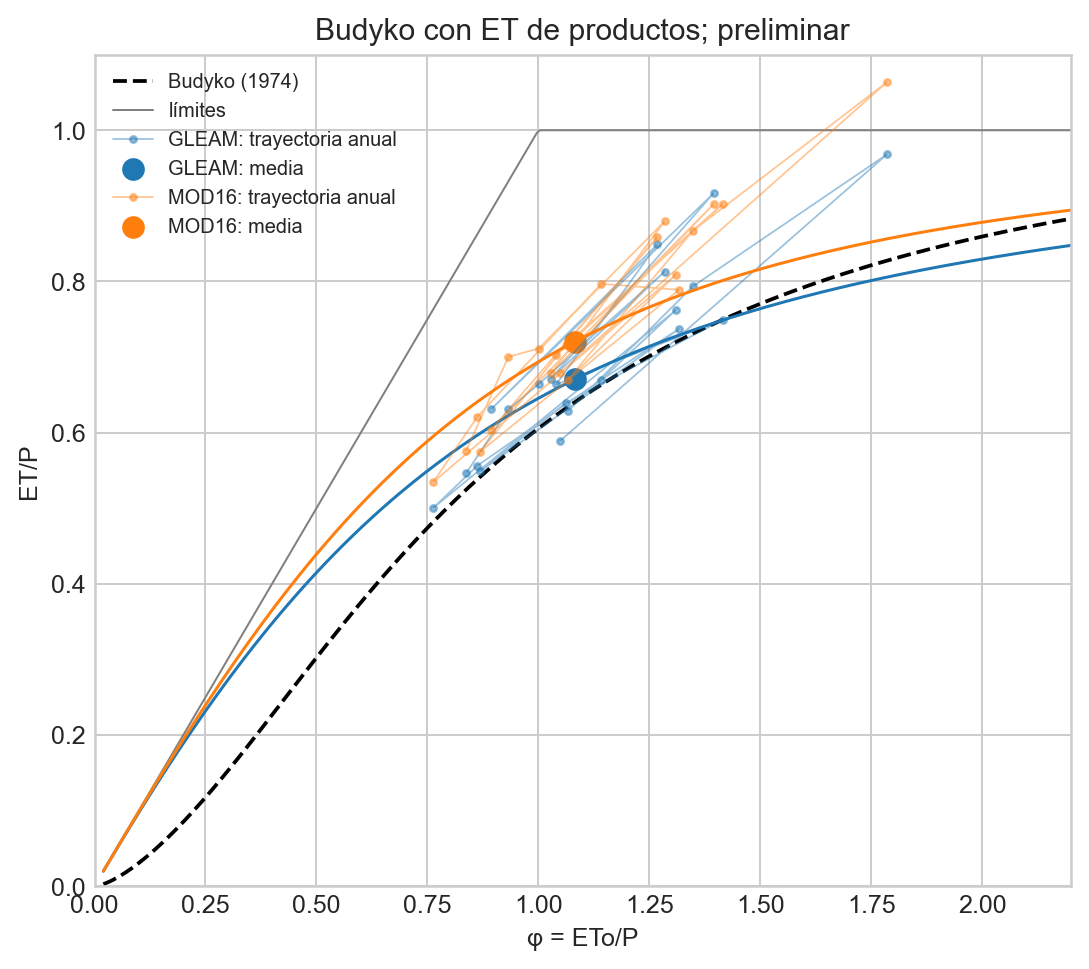
\includegraphics[width=\linewidth,height=0.72\textheight,keepaspectratio]{1_3_regimen_evaporativo/figuras/1_3_integracion_1_3_3_Budyko_ET_real.png}
\end{minipage}

% ---------------------------------------------------------------- 6
\slide{Punto 1 · Régimen evaporativo}{Manda la energía en la temporada húmeda y el agua en la seca}
\begin{minipage}[c]{0.58\linewidth}
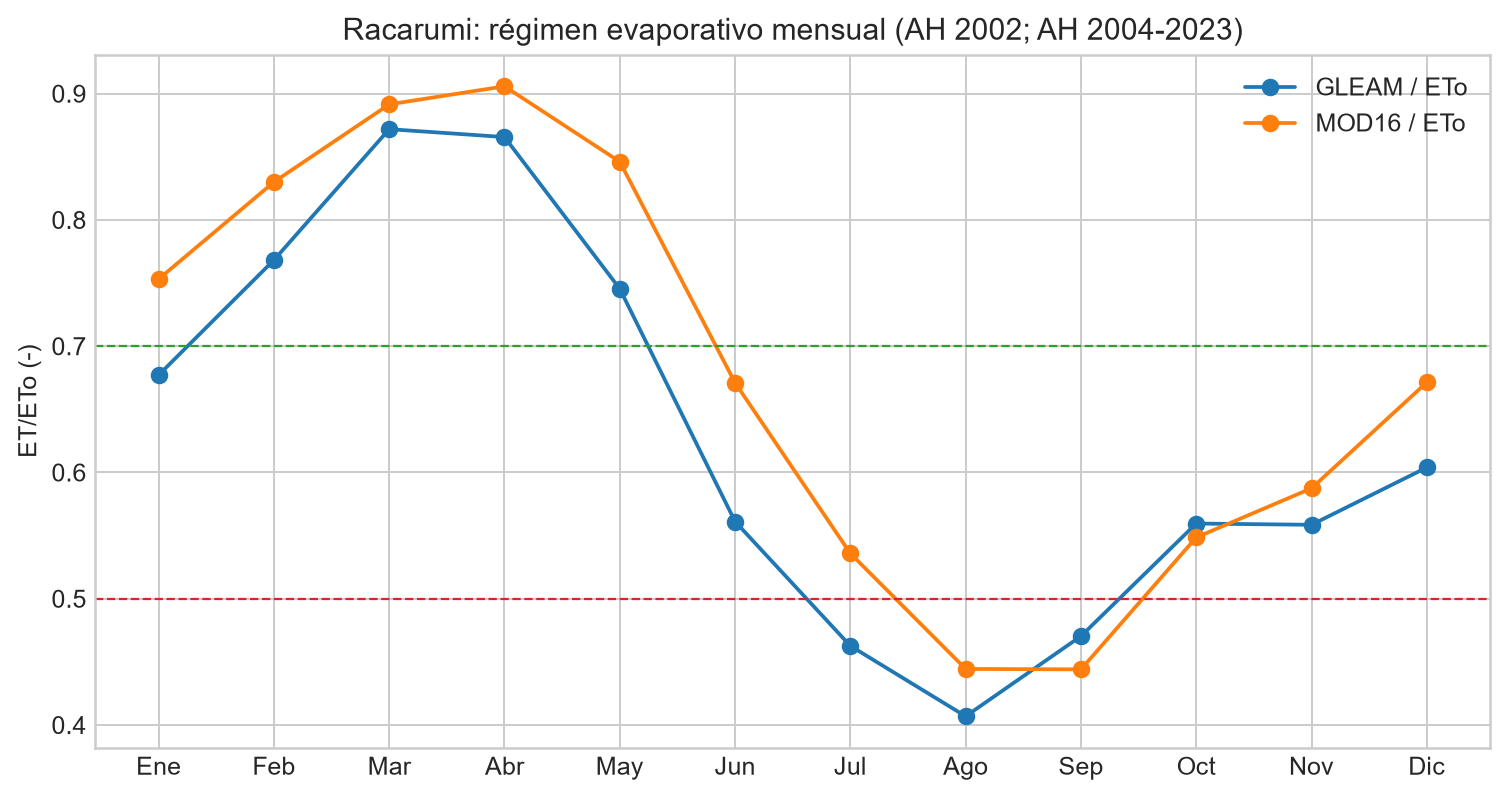
\includegraphics[width=\linewidth,height=0.72\textheight,keepaspectratio]{1_3_regimen_evaporativo/figuras/1_3_integracion_1_3_1_ET_sobre_ETo_mensual.png}
\end{minipage}\hfill
\begin{minipage}[c]{0.38\linewidth}
\large
\begin{itemize}
\item Ene--abr: $ET/\mathrm{ETo}$ = \EToHumMin--\EToHumMax
\item Jun--sep: \EToSecMin--\EToSecMax, con $ET>P$; el agua sale del suelo (0,39 $\to$ 0,26 m$^3$/m$^3$)
\item Budyko: $\phi$ = \PhiAr, en la transición; $\omega$ = \OmG--\OmM
\item Años secos: más demanda (relación complementaria)
\end{itemize}
\end{minipage}

% ---------------------------------------------------------------- 7
\slide{Punto 1 · Cambio y paisaje}{La demanda crece; la altura ordena la evapotranspiración}
\begin{minipage}[t]{0.48\linewidth}
\centering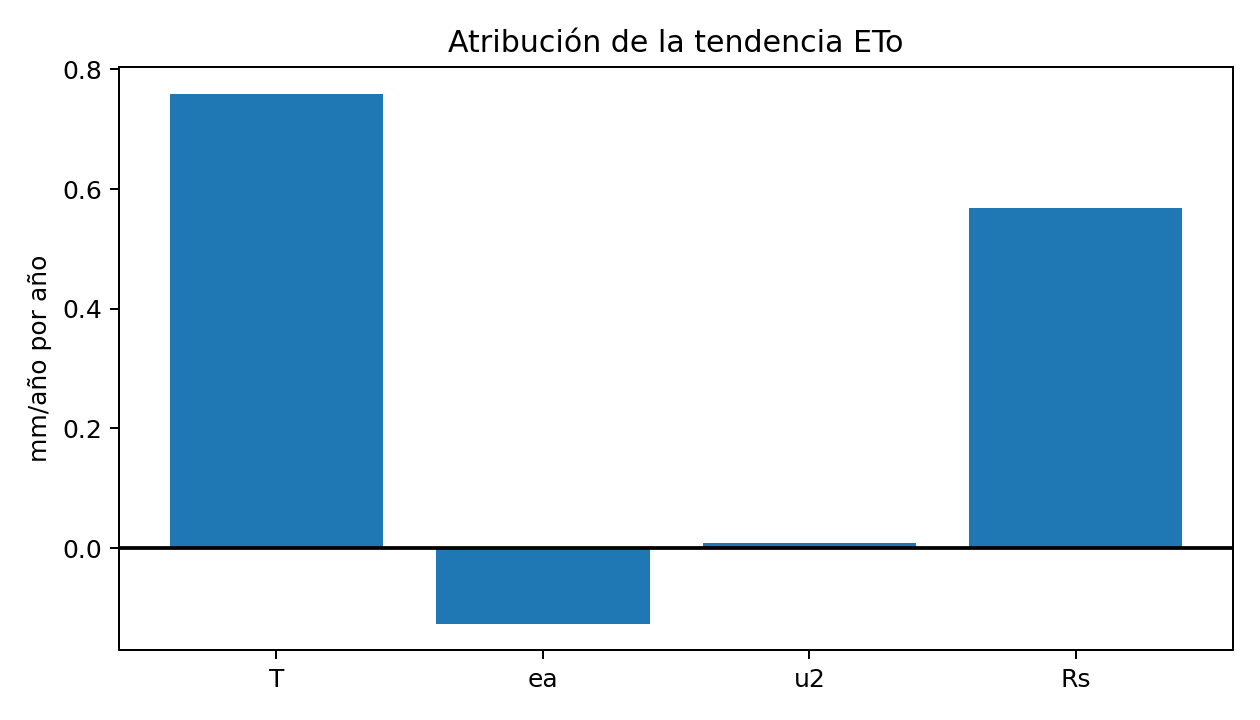
\includegraphics[width=\linewidth,height=0.55\textheight,keepaspectratio]{1_4_cambios_demanda_evaporativa/figuras/1_4_2_contribuciones.png}\raggedright\\[4pt]
\large ETo: \textbf{+\TendETo\ mm/año por año} ($p$ = \pETo)\\
Temperatura +\AtrT, radiación +\AtrRs, humedad \AtrEa
\end{minipage}\hfill
\begin{minipage}[t]{0.48\linewidth}
\centering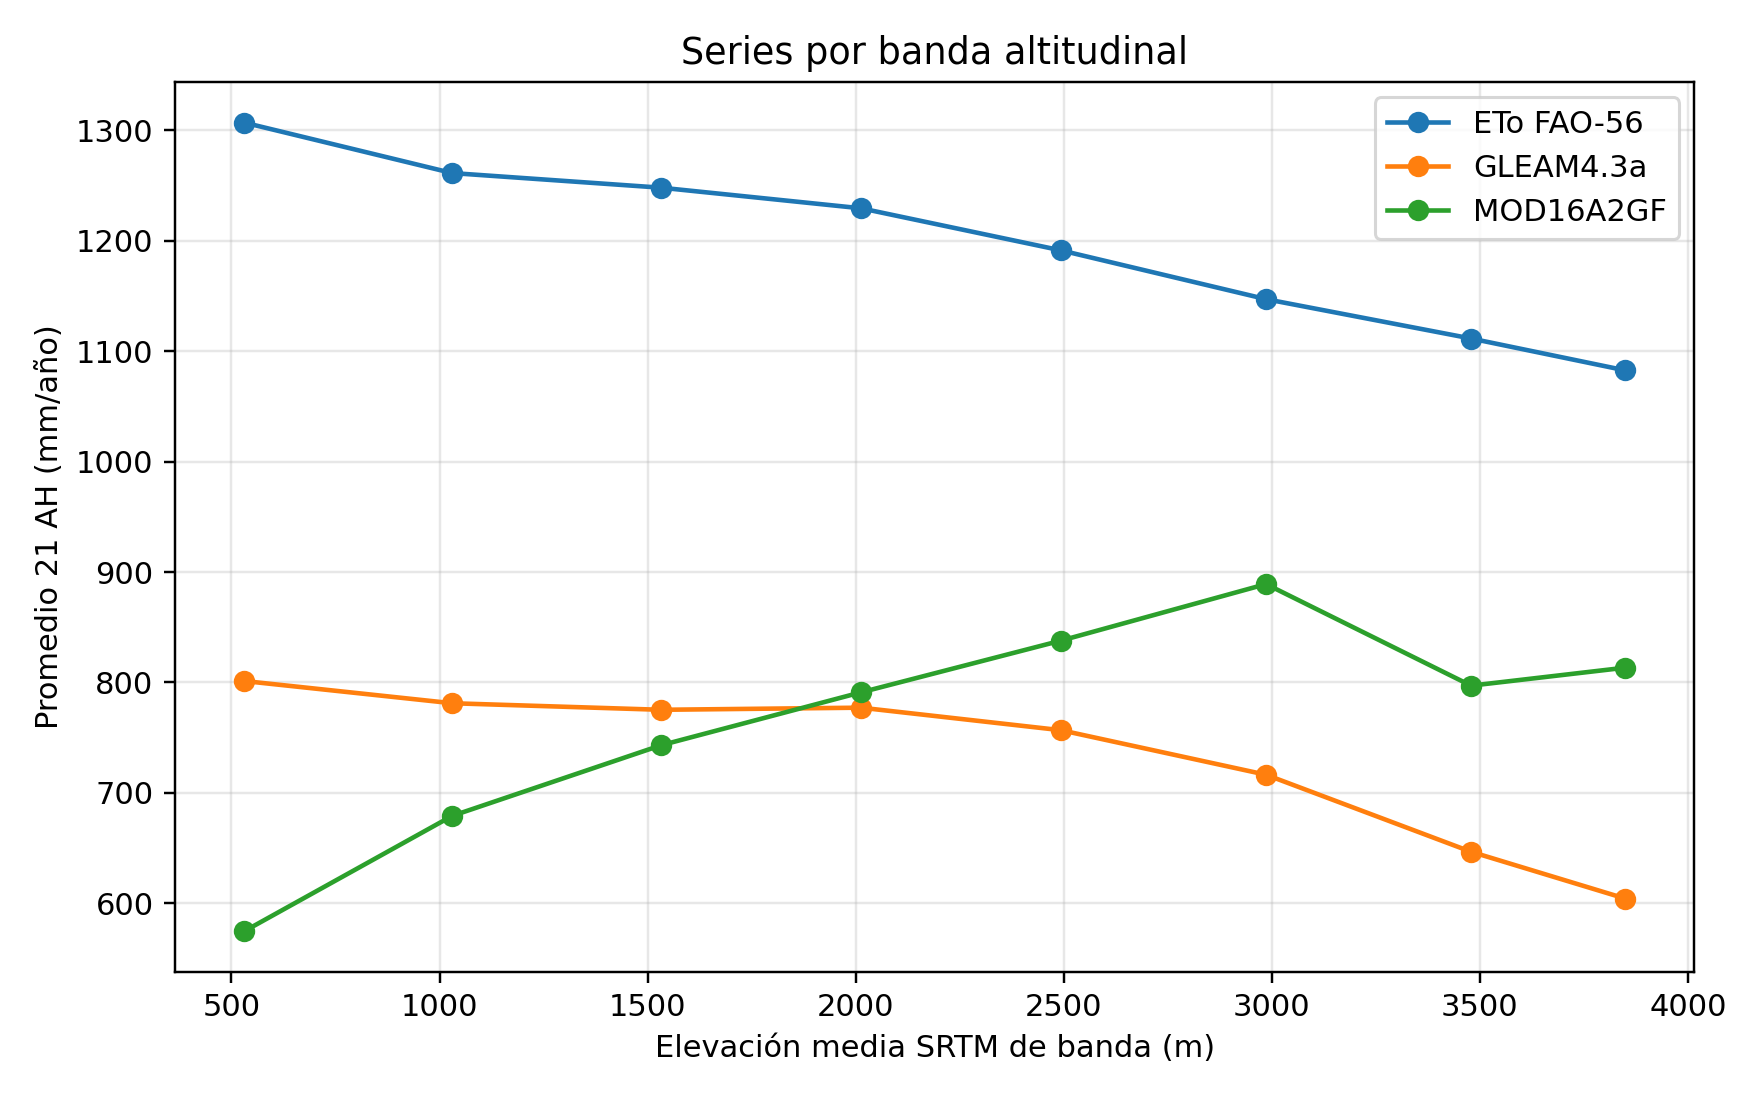
\includegraphics[width=\linewidth,height=0.55\textheight,keepaspectratio]{1_5_paisaje/1_5_gradiente_multianual_productos.png}\raggedright\\[4pt]
\large La ETo baja con la altura (\EToBajo $\to$ \EToAlto\ mm)\\
MOD16 alcanza su máximo a media ladera (\ModMaxBanda)
\end{minipage}

% ---------------------------------------------------------------- 8
\slide{Punto 2 · Datos y métodos}{De la serie de 10 minutos a la IDF}
\large
\begin{minipage}[t]{0.47\linewidth}
\begin{itemize}
\item Máximos anuales con ventanas móviles, 10 min a 24 h; año hidrológico octubre--septiembre
\item Corrección de Weiss: $\times$\WeissDiez\ en 10 min
\item Gumbel, GEV y log-Pearson III por momentos, L-momentos y máxima verosimilitud
\end{itemize}
\end{minipage}\hfill
\begin{minipage}[t]{0.47\linewidth}
\begin{itemize}
\item Con $N$ = 20 la GEV por máxima verosimilitud es inestable $\Rightarrow$ \textbf{GEV-GMLE} (Martins y Stedinger, 2000)
\item Bootstrap de \NBoot\ réplicas por años completos
\item IDF de Koutsoyiannis: error máximo de \IDFerr\,\%, $R^2$ = \IDFrdos
\end{itemize}
\end{minipage}

% ---------------------------------------------------------------- 9
\slide{Punto 2 · Control de calidad}{El evento de 2013 es real: una celda convectiva sobre la estación}
\begin{minipage}[c]{0.62\linewidth}
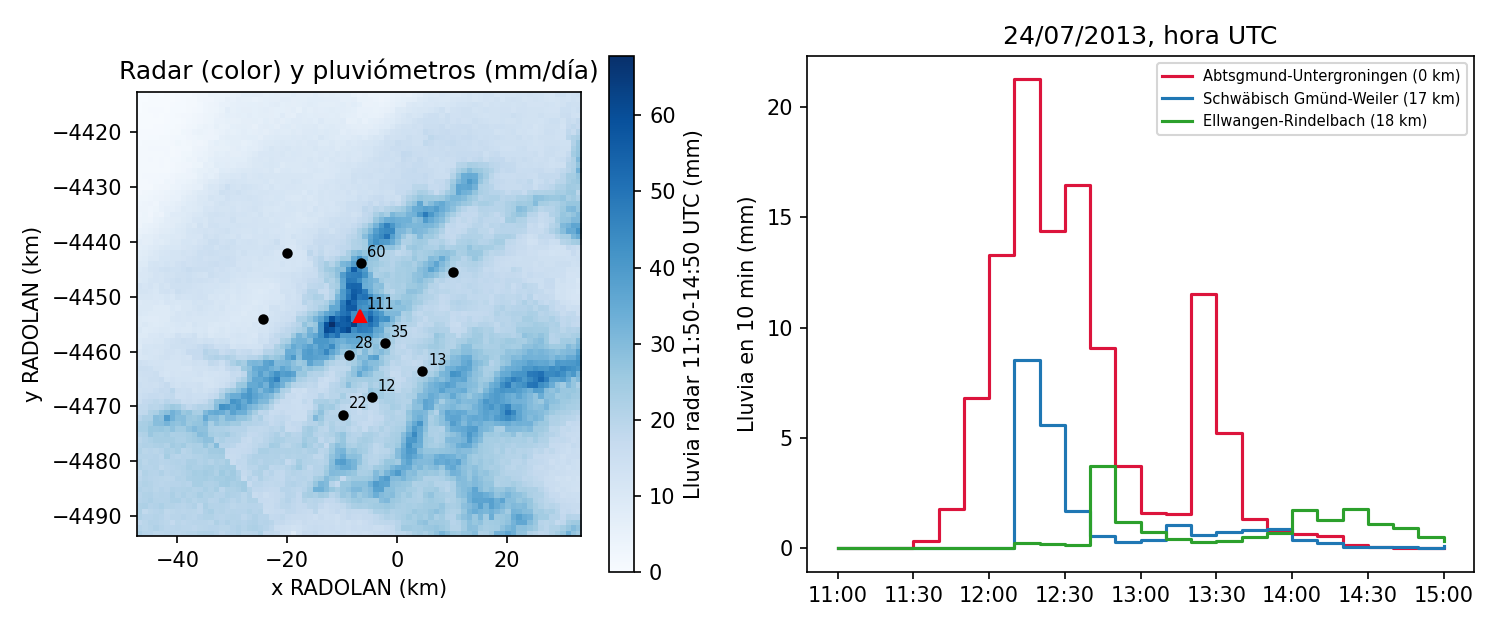
\includegraphics[width=\linewidth,height=0.72\textheight,keepaspectratio]{evento_2013_contraste.png}
\end{minipage}\hfill
\begin{minipage}[c]{0.35\linewidth}
\cifra{81 mm en 1 h}{24/07/2013, la mayor del registro}\\[10pt]
\large
\begin{itemize}
\item Radar: \EvRadarEst\ mm/h en la celda de la estación
\item Bühlerzell (\EvBuhlerKm\ km): \EvBuhler\ mm en el día
\item Vecinas a 17 km: \EvGmundHora\ y \EvEllwHora\ mm/h
\end{itemize}
\end{minipage}

% ---------------------------------------------------------------- 10
\slide{Punto 2 · Curvas IDF}{La cola local es más pesada que KOSTRA, en parte por 2013}
\begin{minipage}[c]{0.55\linewidth}
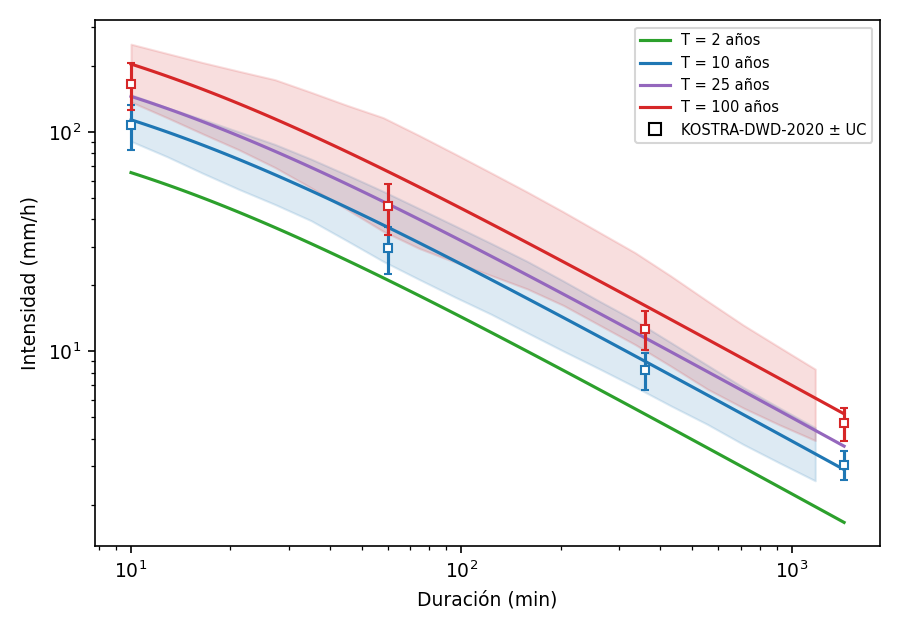
\includegraphics[width=\linewidth,height=0.72\textheight,keepaspectratio]{idf_bandas_kostra.png}
\end{minipage}\hfill
\begin{minipage}[c]{0.41\linewidth}
\large 1 h, $T$ = 100 años:\\[6pt]
\begin{tabular}{lr}
Estación local & \textbf{\VecPropQcien\ mm}\\
Vecinas (23 años) & \VecGmundQcien\ y \VecEllwQcien\ mm\\
Local sin 2013 & \SinHoraTcien\ mm\\
KOSTRA-DWD-2020 & \KosHoraTcien\ $\pm$ \KosUCHoraTcien\,\%
\end{tabular}\\[12pt]
En 10 min, la duración de diseño, la IDF local queda dentro de la incertidumbre de KOSTRA
\end{minipage}

% ---------------------------------------------------------------- 11
\slide{Punto 2 · Problema A}{El riesgo real supera al nominal: se recomienda 1,05 m}
\begin{minipage}[c]{0.5\linewidth}
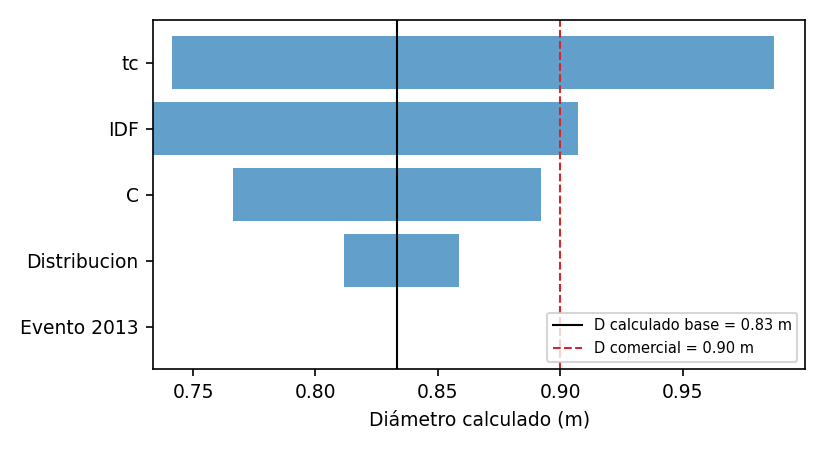
\includegraphics[width=\linewidth,height=0.6\textheight,keepaspectratio]{tornado_2_4A.png}\\[4pt]
\large Mayor incertidumbre: $t_c$, luego la IDF y $C$
\end{minipage}\hfill
\begin{minipage}[c]{0.46\linewidth}
\large $t_c$ (SCS) = \tcSCS\ min · $C$ = \Cpre · $T$ = \Tdis\ años\\
$Q_p$ = \Qp\ m$^3$/s $\Rightarrow$ $D$ = \Dcalc\ m $\Rightarrow$ comercial \Dcom\ m\\[8pt]
Monte Carlo con \Dcom\ m: $T$ efectivo $\approx$ \Teff\ años\\[10pt]
\cifra{\Drec\ m}{$T$ efectivo $\approx$ \TeffRec\ años · riesgo en \Vida\ años \RiesgoEffRec\,\%}
\end{minipage}

% ---------------------------------------------------------------- 12
\slide{Punto 2 · Problema B}{El tanque devuelve el pico urbanizado al nivel previo}
\centering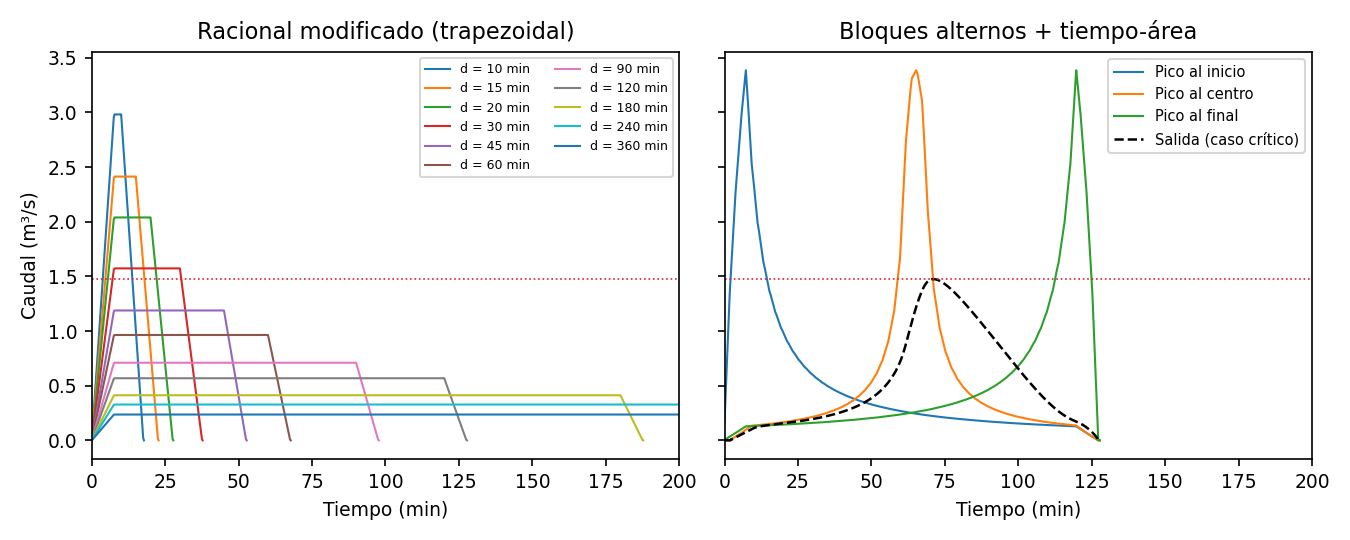
\includegraphics[width=0.92\linewidth,height=0.5\textheight,keepaspectratio]{hidrogramas_tanque_2_4B.png}\par\vspace{6pt}
\raggedright
\begin{minipage}[t]{0.6\linewidth}
\large
\begin{itemize}
\item Urbanizado: $C$ \Cpre\ $\to$ \Curb; $t_c$ \tcSCS\ $\to$ \tcUrb\ min; salida $\le Q_{pre}$ = \Qpre\ m$^3$/s
\item Volumen: trapezoidal \VolTrap\ m$^3$; bloques alternos \VolCentro\ m$^3$ (pico al centro)
\end{itemize}
\end{minipage}\hfill
\begin{minipage}[t]{0.36\linewidth}
\cifra{\LadoTanque\,$\times$\,\LadoTanque\,$\times$\,\Hutil\ m}{Tanque recomendado · orificio de \DOrif\ m}
\end{minipage}

% ---------------------------------------------------------------- 13
\slide{Cierre}{Qué nos llevamos}
\Large
\begin{itemize}[itemsep=12pt]
\item La \textbf{radiación} controla la demanda; un método solo térmico exagera el calentamiento.
\item La cuenca devuelve \textbf{algo más de la mitad} de su lluvia, y el error viene de la lluvia.
\item \textbf{Energía} en la temporada húmeda, \textbf{agua} en la seca: el suelo sostiene la ET.
\item Con 20 años de registro, el \textbf{riesgo efectivo} debe guiar el diseño, no el nominal.
\item Límites: 90\,\% de cobertura de ERA5-Land, trasvases sin cuantificar, salida sintética.
\end{itemize}
\end{document}
